\subsection{Protocol Selection}

\subsubsection{Requirements}
\paragraph{Flight Control}
\begin{table}[h]
\centering
\begin{tabular}{|c|c|c|c|c|} 
\hline
\textbf{Purpose}&\textbf{Frequency (Hz)}&\textbf{Message Size(bits)}&\textbf{Quantity}&\textbf{Bandwidth (kbps)}\\
\hline
ESC Duty Cycle&400&16&4&25.6\\
ESC Telemetry&10&64&4&2.56\\
Fault ESC Telemetry&400&64&4&102.4\\
Imaging Location&100&48&1&4.8\\
BMS Telemetry&10&32&1&0.32\\
GNSS location&10&48&2&0.96\\
Collision Detection&100&16&2&3.2\\
GNSS Correction&1&500&1&0.5\\
\hline
\end{tabular}
\caption{Required Standard Messages}
\label{tab:device_comms_requirementsl}
\end{table}


The flight controller and its associated devices are the core of the communication network as it connects all the devices required to fly. Table \ref{tab:device_comms_requirementsl} shows the standard, non imaging, messages during flight. If using 32 bit messages, \ref{tab:device_comms_requirementsl} corresponds to a standard required capacity of 61.1 kbps that. However, when carrying out actuator fault quantification it should support telemetry messages specified in \ref{tab:fault_messages} requiring an additional 51.2 kbps. To future proof the system against future module additions, greater length messages or faster messaging speeds, it should then have at least an additional 50 kbps. This brings the total capacity required to 162.3 kbps.
\subsubsection{Options}
\begin{table}[h]
\centering
\begin{tabular}{|c|c|c|c|c|c|c|} 
\hline
\textbf{Protocol} & \textbf{Speed} & \textbf{Complexity} & \textbf{Power Draw} & \textbf{Noise Tolerance} & \textbf{Cost} & \textbf{Use Case} \\ 
\hline 
CAN FD & 5 Mbps & Medium & Medium & High & Medium & Bus \\ 
FlexRay & 10 Mbps & High & High & High & High & Bus \\ 
I$^2$C & 400 Kbps & Low & Low & Low & Low & Sensors \\ 
SPI & 100 Mbps & Medium & Low & Medium & Low & Sensors \\ 
UART & 1 Mbps & Low & Low & Low & Low & Sensors \\ 
Ethernet & 1 Gbps & Medium & Medium & High & Medium & Imaging \\ 
\hline 
\end{tabular}
\caption{Communication Protocols}
\label{tab:communication_options}
\end{table}

\subsubsection{Communication between Modules}
\paragraph{Architecture}
Star architectures consist of a central node directly connected to all the relevant devices. This creates a single point of failure on the star centre, in this case the flight controller. Federated architectures and distributed architectures, remove this dependency on a single point and therefore represent more complex but more resilient networks. A compromise used in this case is that the custom \gls{GNSS} modules deployed also have the capability of control to execute landing and return to safety. This means that if the flight controller \gls{MCU} malfunctions the drone can safely land or return to safety.  
\paragraph{Bus Selection}
FlexRay has some clear advantages including built in redundancy and higher data transfer speeds. However, due to its added complexity, cost and the fact it is compatible with far fewer components a \gls{CAN} bus is the better option. This may change if the data transfer rates needed to increase or if the technology behind FlexRay becomes cheaper and more widespread. Further, there are two key options for \gls{CAN}, time triggered or flexible data. Time triggered is an attractive option for this application as the control systems run and constant frequency however, flexible data is more widespread and allows for better telemetry. This is because, when there is a fault being detected, the sampling frequency should increase so that it can be quantified with higher accuracy.
\paragraph{CAN bus network}
Devices should be distributed on the lines as in \ref{fig:CAN_bus}, the redundant modules are on separate lines and the modules with no redundancy are connected to both lines. This means that if a \gls{GNSS} module has a catastrophic failure the other line has all the safety critical nodes and is intact. It however, does not mitigate against catastrophic failure of the non-redundant modules.
 \begin{figure}[h!]
 \centering
  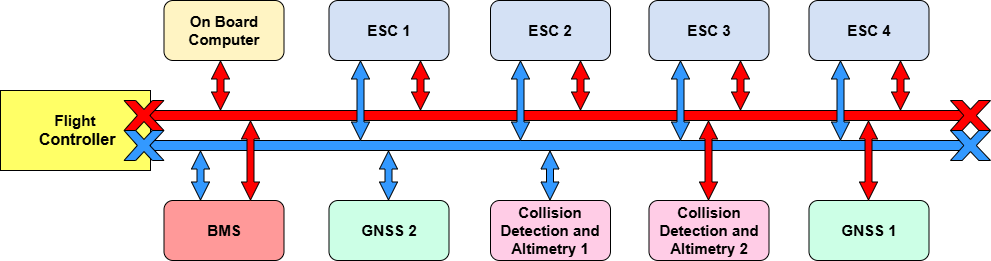
\includegraphics[width=1\textwidth]{figs/Thomas/Intra Communication/CAN bus.png}
 \caption{CAN bus layout}
 \label{fig:CAN_bus}
 \end{figure}
\paragraph{}

\subsubsection{Communication with sensors}
\paragraph{High Speed Sensors}
The simple but high speed \gls{SPI} protocol should be used whenever possible. This is because it is widely supporting by commercially available sensors and \gls{MCU}s. This, combined with its high data capacity means it is the best option for high speed sensor communication. 
\paragraph{Low Speed Sensors}
Both \gls{UART} and \gls{I$^2$C} are widely supported, both are simple and effective however, \gls{UART} is simpler therefore on non-complex modules is used where possible. However, if board-space because a limitation \gls{I$^2$C} should be used.
\paragraph{Memory Devices}
MicroSD and SD cards can communicate with \gls{SPI} or \gls{SDIO}. \gls{SDIO} is the native application and is faster and more effective, however, it requires pins that are often more widely distributed on \gls{MCU}s making it more difficult to design with. Therefore, for the Flight Controller \gls{SPI} was used as the data transfer rates for recording the state vector need not exceed 100 Hz and therefore do not require the higher data transfer rates from \gls{SDIO}. However, while recording imaging data on the main computers SD card, \gls{SDIO} should be used in order to support the ultra high writing speeds required. 
\paragraph{Imaging Sensors}
The imaging sensors require very high data transfer rates and are not safety critical. They are therefore not included on the \gls{CAN} bus but instead directly connect to the onboard computer using Ethernet. 

\paragraph{Debugger}
Debugging is possible using the \gls{CAN} bus at a system level but for in depth on board debugging that might be required for failure analysis or uploading code to boards should also be available. This can be done using \gls{UART} however, it is slower and has less functionality than using a \gls{SWD}. \gls{SWD} allows for real-time variable inspection and breakpoints. Therefore, for system wide debugging the \gls{CAN} bus will be used, and for onboard debugging a \gls{SWD} will be used.

\subsubsection{High Level Application Protocol}
\paragraph{Relevance}
A single high level protocol being used across all components makes the drone more adaptable and makes hiring developers easier. This is because a single skill-set can interact with the entire system. This however, comes with challenges due to the mapping sensors operating on different hardware to the other modules.
\paragraph{Cyphal}
Cyphal provides the perfect solution for this as it can be used over all major communication hardware. It was originally developed for, and is compatible with, \gls{UAV} components, and has since expanded to include further functionalities including Ethernet and \gls{USB}. This ensures that the system is easier to upgrade.
